\subsection{Interfaccia REST}
Di seguito sono elencate le risorse REST associate al tipo di metodo che è possibile richiedere su di esse e i permessi richiesti per poter effettuare la richiesta.
Le tipologie di permessi sono:
\begin{itemize}
	\item Utente non autenticato: risorsa che può essere richiesta da qualsiasi utente;
	\item Utente autenticato: risorsa che può essere richiesta solo da utenti autenticati;
	\item Utente proprietario: risorsa che può essere richiesta solo da utenti proprietari di un progetto.
\end{itemize}

\begin{table}[h]
	\begin{tabular}{|p{0.5\textwidth}|p{0.15\textwidth}|p{0.35\textwidth}|}
		\toprule
		
		\textbf{Chiamata} & \textbf{Tipo risorsa}  & \textbf{Tipo utente} \\
		\bottomrule
	\end{tabular}\\	
\end{table}

\begin{table}[h]
	\begin{tabular}{|p{0.5\textwidth}|p{0.15\textwidth}|p{0.35\textwidth}|}
		\toprule
		\textbf{/login}	& \textbf{POST} & \textbf{Utente non autenticato} \\ \midrule
		\multicolumn{3}{|c|}{Crea una nuova sessione associata all'utente, corrisponde all'azione di login.} \\
		\bottomrule
	\end{tabular}\\
	\par\bigskip
	
	\begin{tabular}{|p{0.5\textwidth}|p{0.15\textwidth}|p{0.35\textwidth}|}
		\toprule
		\textbf{/logout} & \textbf{DELETE} & \textbf{Utente autenticato, Utente proprietario} \\ \midrule
		\multicolumn{3}{|c|}{Elimina la sessione associata all'utente, corrisponde all'azione di logout.} \\
		\bottomrule
	\end{tabular}\\
	\par\bigskip
	
	\begin{tabular}{|p{0.5\textwidth}|p{0.15\textwidth}|p{0.35\textwidth}|}
		\toprule
		\textbf{/register} & \textbf{POST} & \textbf{Utente non autenticato} \\ \midrule
		\multicolumn{3}{|c|}{Crea una richiesta di registrazione.} \\
		\bottomrule
	\end{tabular}\\
	\par\bigskip
	
	\begin{tabular}{|p{0.5\textwidth}|p{0.15\textwidth}|p{0.35\textwidth}|}
		\toprule
		\textbf{/forgotpassword} & \textbf{POST} & \textbf{Utente non autenticato} \\ \midrule
		\multicolumn{3}{|c|}{Crea una richiesta di recupero password.} \\
		\bottomrule
	\end{tabular}\\
	\par\bigskip
	
	\begin{tabular}{|p{0.5\textwidth}|p{0.15\textwidth}|p{0.35\textwidth}|}
		\toprule
		\textbf{/search} & \textbf{GET} & \textbf{Utente non autenticato, Utente autenticato, Utente proprietario} \\ \midrule
		\multicolumn{3}{|c|}{Restituisce i risultati di una ricerca.} \\
		\bottomrule
	\end{tabular}\\
	\par\bigskip
	
	\begin{tabular}{|p{0.5\textwidth}|p{0.15\textwidth}|p{0.35\textwidth}|}
		\toprule
		\textbf{/projects} & \textbf{GET} & \textbf{Utente proprietario} \\ \midrule
		\multicolumn{3}{|c|}{Restituisce la lista di tutti i progetti del relativo utente.} \\
		\bottomrule
		\textbf{/projects} & \textbf{POST} & \textbf{Utente proprietario} \\ \midrule
		\multicolumn{3}{|c|}{Crea un nuovo progetto.} \\
		\bottomrule
	\end{tabular}
\end{table}
\newpage

\begin{table}[H]
	\begin{tabular}{|p{0.5\textwidth}|p{0.15\textwidth}|p{0.35\textwidth}|}
		\toprule
		\textbf{/projects/project/\{id\}} & \textbf{GET} & \textbf{Utente proprietario} \\ \midrule
		\multicolumn{3}{|c|}{Restituisce i dati del progetto con id project/\{id\}.} \\ \midrule
		\textbf{/projects/project/\{id\}} & \textbf{PUT} & \textbf{Utente proprietario} \\ \midrule
		\multicolumn{3}{|c|}{Modifica i dati del progetto con id project/\{id\}.} \\ \midrule
		\textbf{/projects/project/\{id\}} & \textbf{DELETE} & \textbf{Utente proprietario} \\ \midrule
		\multicolumn{3}{|c|}{Elimina il progetto con id project/\{id\}.} \\
		\bottomrule
	\end{tabular}
	\\ \par\bigskip
	
	\begin{tabular}{|p{0.5\textwidth}|p{0.15\textwidth}|p{0.35\textwidth}|}
		\toprule
		\textbf{/projects/project/\{id\}/infographic} & \textbf{GET} & \textbf{Utente proprietario} \\ \midrule
		\multicolumn{3}{|c|}{Restituisce i dati dell'infografica del progetto con id project/\{id\}.} \\
		\bottomrule
		\textbf{/projects/project/\{id\}/infographic} & \textbf{POST} & \textbf{Utente proprietario} \\ \midrule
		\multicolumn{3}{|c|}{Crea un'infografica relativa al progetto con id project/\{id\}.} \\
		\bottomrule
		\textbf{/projects/project/\{id\}/infographic} & \textbf{DELETE} & \textbf{Utente proprietario} \\ \midrule
		\multicolumn{3}{|c|}{Elimina l'infografica relativa al progetto con id project/\{id\}.} \\
		\bottomrule
	\end{tabular}\\
	\par\bigskip
	
	\begin{tabular}{|p{0.5\textwidth}|p{0.15\textwidth}|p{0.35\textwidth}|}
		\toprule
		\textbf{/projects/project/\{id\}/presentation} & \textbf{GET} & \textbf{Utente proprietario} \\ \midrule
		\multicolumn{3}{|c|}{Restituisce i dati della presentazione del progetto con id project/\{id\}.} \\
		\bottomrule
		\textbf{/projects/project/\{id\}/presentation} & \textbf{POST} & \textbf{Utente proprietario} \\ \midrule
		\multicolumn{3}{|c|}{Crea una presentazione relativa al progetto con id project/\{id\}.} \\
		\bottomrule
		\textbf{/projects/project/\{id\}/presentation} & \textbf{DELETE} & \textbf{Utente proprietario} \\ \midrule
		\multicolumn{3}{|c|}{Elimina la presentazione relativa al progetto con id project/\{id\}.} \\
		\bottomrule
	\end{tabular}\\
	\par\bigskip
	
	\begin{tabular}{|p{0.5\textwidth}|p{0.15\textwidth}|p{0.35\textwidth}|}
		\toprule
		\textbf{/projects/project/\{id\}/presentation
			/slide/\{id\}/components} & \textbf{GET} & \textbf{Utente proprietario} \\ \midrule
		\multicolumn{3}{|p{1.0\textwidth}|}{Restituisce la lista dei componenti della slide con id slide/\{id\} nella presentazione del progetto con id project/\{id\}.} \\
		\bottomrule
	\end{tabular}\\
	\par\bigskip
	\begin{tabular}{|p{0.5\textwidth}|p{0.15\textwidth}|p{0.35\textwidth}|}
		\toprule
		\textbf{/projects/project/\{id\}/presentation
			/slide/\{id\}/components/component/\{id\}} & \textbf{POST} & \textbf{Utente proprietario} \\ \midrule
		\multicolumn{3}{|p{1.0\textwidth}|}{Crea la componente di id component/\{id\} nella slide con id slide/\{id\} della presentazione relativa al progetto con id project/\{id\}.} \\
		\bottomrule
		\textbf{/projects/project/\{id\}/presentation
			/slide/\{id\}/components/component/\{id\}} & \textbf{PUT} & \textbf{Utente proprietario} \\ \midrule
		\multicolumn{3}{|p{1.0\textwidth}|}{Modifica la componente di id component/\{id\} nella slide con id slide/\{id\} della presentazione relativa al progetto con id project/\{id\}.} \\
		\bottomrule
		\textbf{/projects/project/\{id\}/presentation
			/slide/\{id\}/components/component/\{id\}} & \textbf{DELETE} & \textbf{Utente proprietario} \\ \midrule
		\multicolumn{3}{|p{1.0\textwidth}|}{Elimina la componente di id component/\{id\} nella slide con id slide/\{id\} della presentazione relativa al progetto con id project/\{id\}.} \\
		\bottomrule
	\end{tabular}	
\end{table}

\newpage
\subsection{Premi::Back-End}
	\subsubsection*{Informazioni sul package}
		\begin{figure}[h]
			\centering
			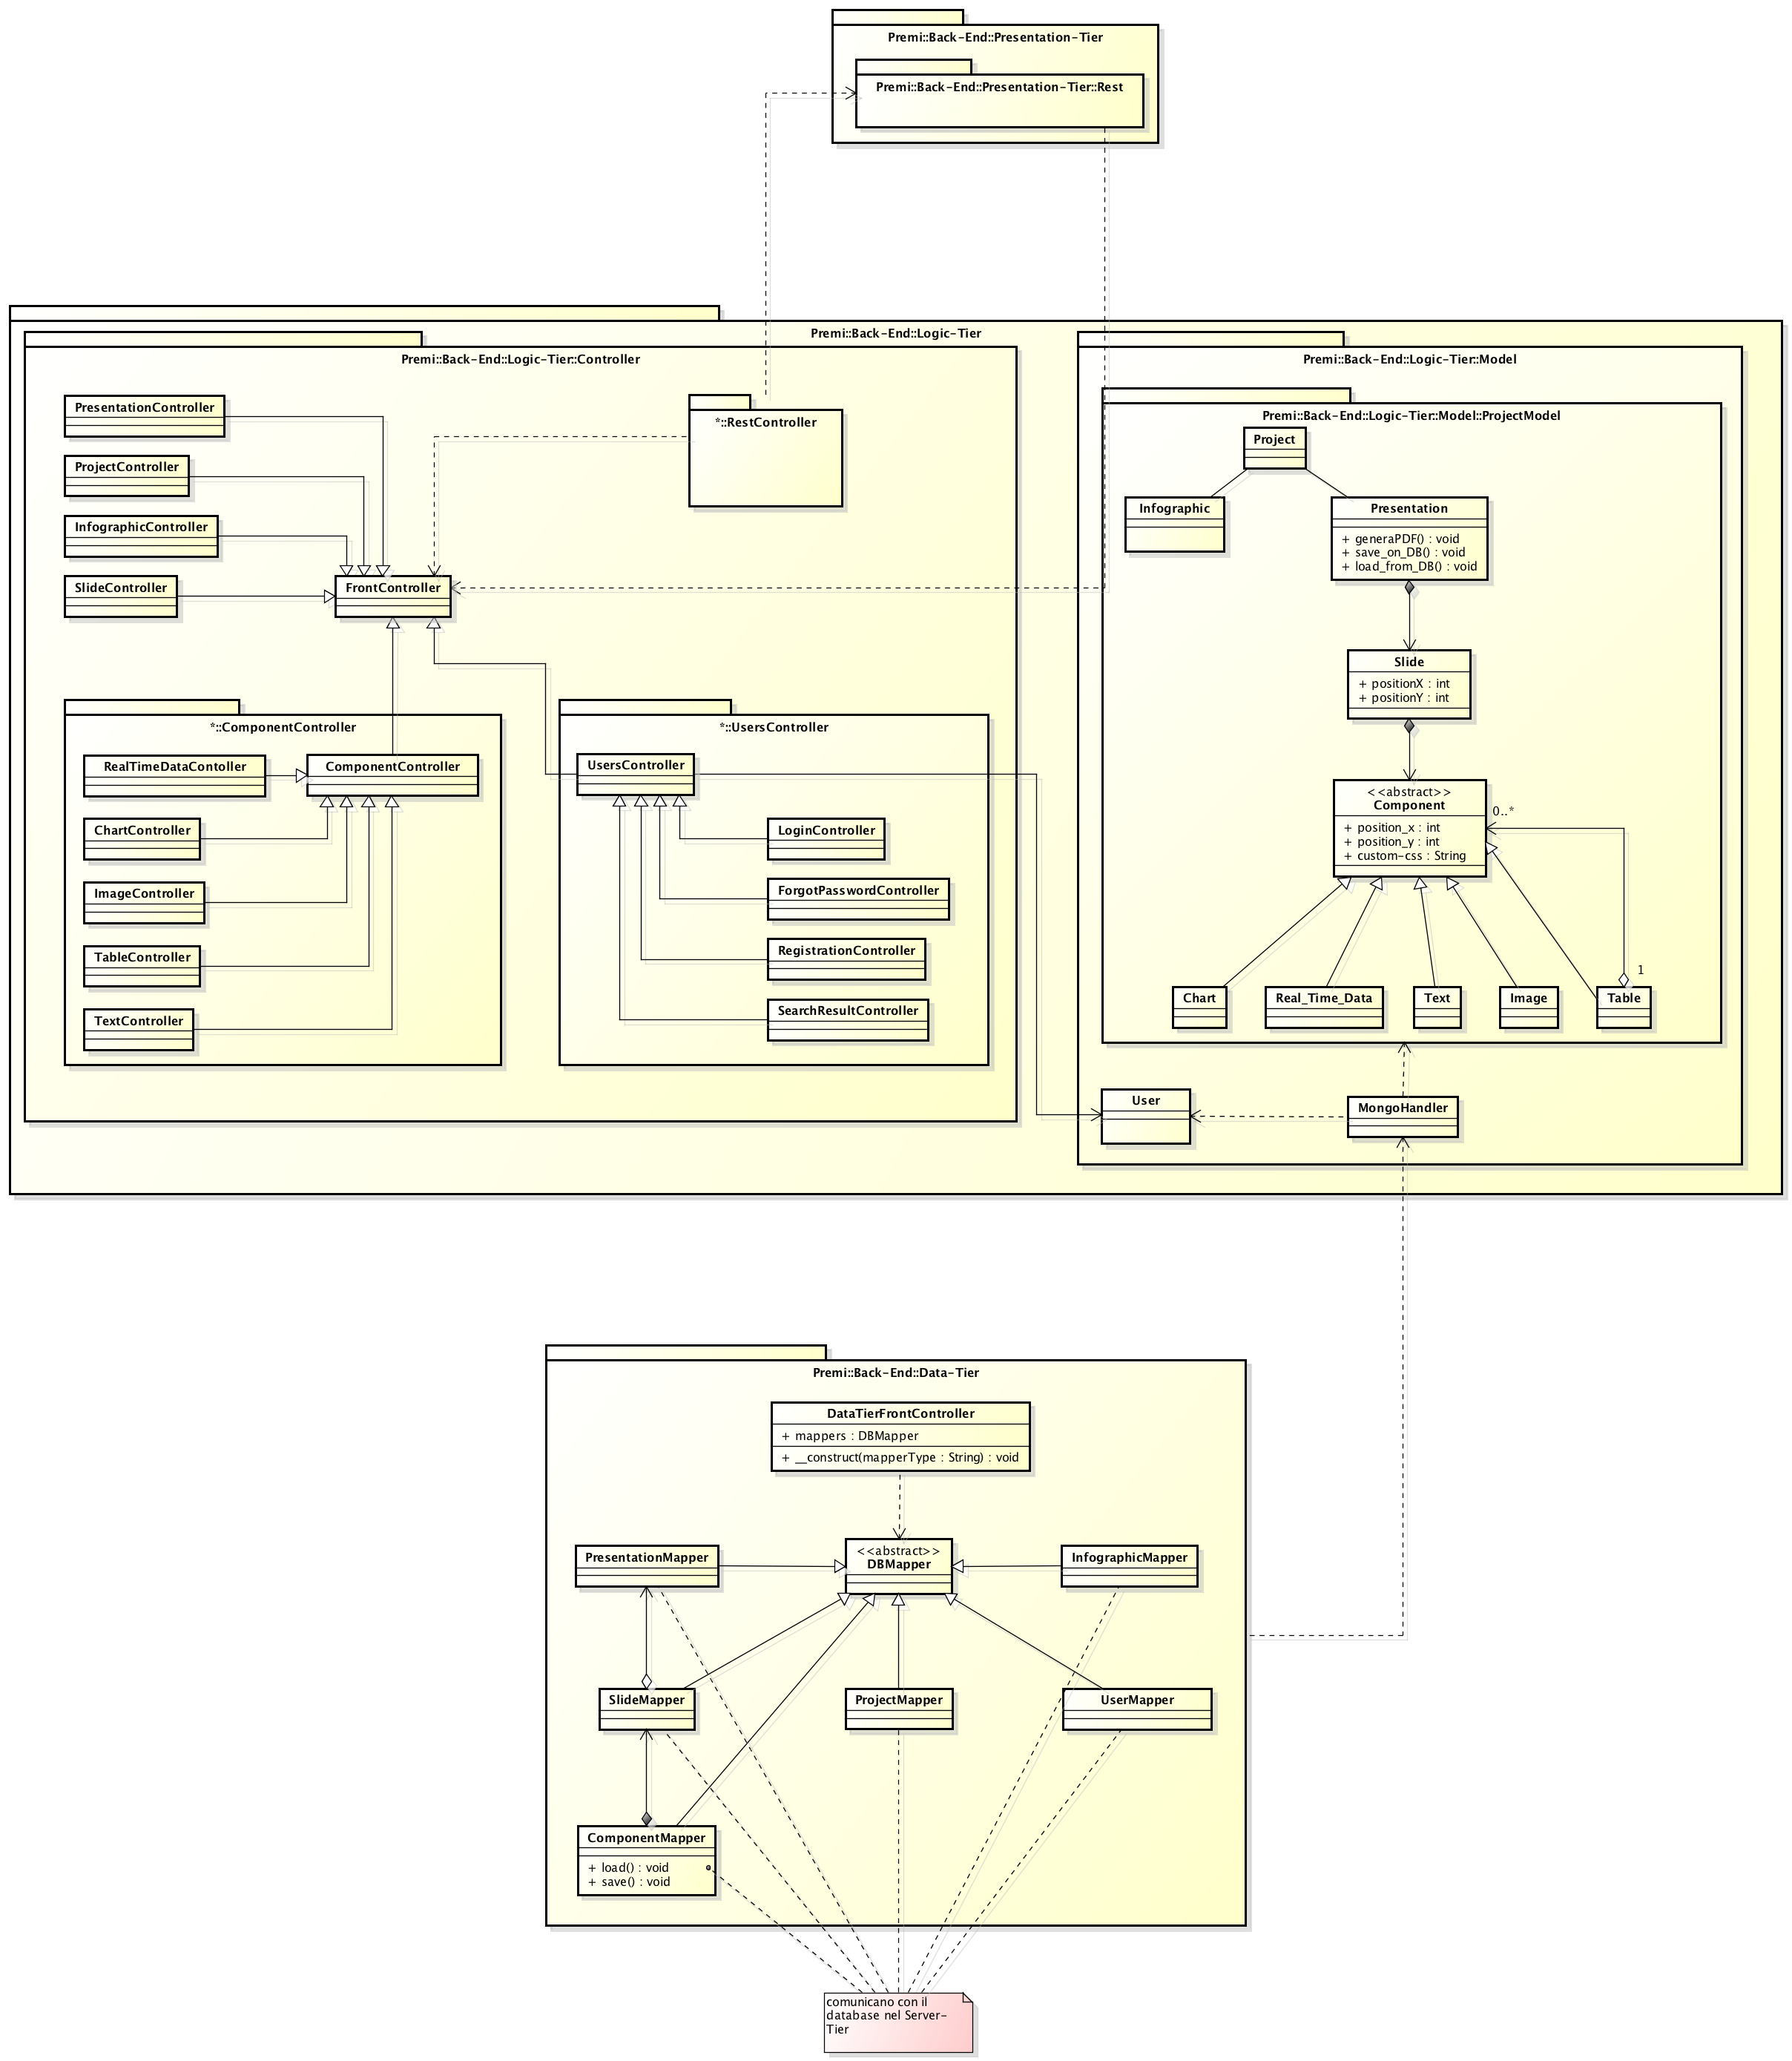
\includegraphics[width=\linewidth]{img/back-end}
			\caption[Premi::Back-End]{Premi::Back-End}
		\end{figure}
		Il package contiene le componenti della parte di back-end dell'applicazione.
		
	\subsubsection*{Package contenuti}
		\begin{itemize}
			\item Premi::Back-End::Presentation-Tier;
			\item Premi::Back-End::Logic-Tier;
			\item Premi::Back-End::Data-Tier.
		\end{itemize}


\subsection{Premi::Back-End::Presentation-Tier}
	\subsubsection*{Informazioni sul package}
		\begin{figure}[h]
			\centering
			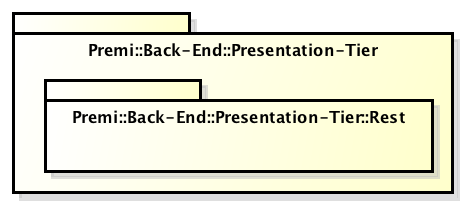
\includegraphics[width=0.5\linewidth]{img/back-end_presentation-tier}
			\caption[Premi::Back-End::Presentation-Tier]{Premi::Back-End::Presentation-Tier}
		\end{figure}
		Il package contiene le componenti necessarie per consentire il funzionamento del servizio REST, in modo tale da rendere possibile l'interfacciamento con il front-end.
		
	\subsubsection*{Package contenuti}
		\begin{itemize}
			\item Premi::Back-End::Data-Tier::REST:
			\begin{itemize}
				\item \textbf{Descrizione}: Il package contiene la struttura necessaria al funzionamento delle chiamate REST da parte del front-end, richiamando i rispettivi controller.
			\end{itemize}
		\end{itemize}
		
		
\subsection{Premi::Back-End::Logic-Tier}
	\subsubsection*{Informazioni sul package}
	\begin{figure}[h]
		\centering
		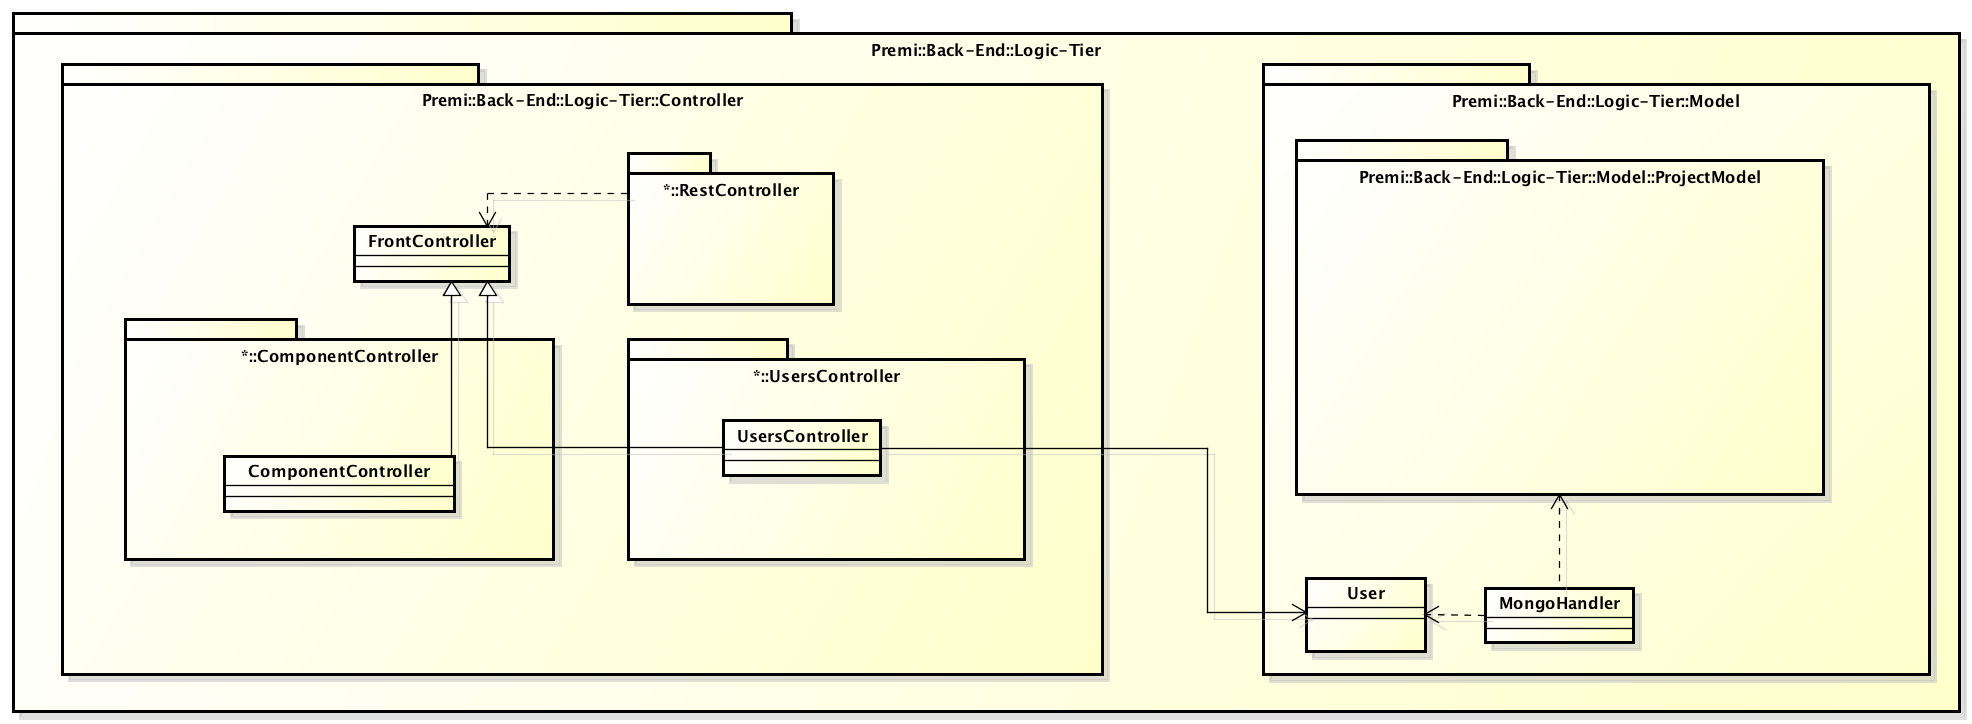
\includegraphics[width=0.9\linewidth]{img/back-end_logic-tier}
		\caption[Premi::Back-End::Logic-Tier]{Premi::Back-End::Logic-Tier}
	\end{figure}
	Il package contiene le componenti che si occupano di ricevere le richieste dal Presentation-Tier e di elaborarle attraverso il controller.
	
	\subsubsection*{Package contenuti}
	\begin{itemize}
		\item Premi::Back-End::Logic-Tier::Controller;
		\item Premi::Back-End::Logic-Tier::Model.
	\end{itemize}


\subsection{Premi::Back-End::Logic-Tier::Controller}
	\subsubsection*{Informazioni sul package}
	\begin{figure}[h]
		\centering
		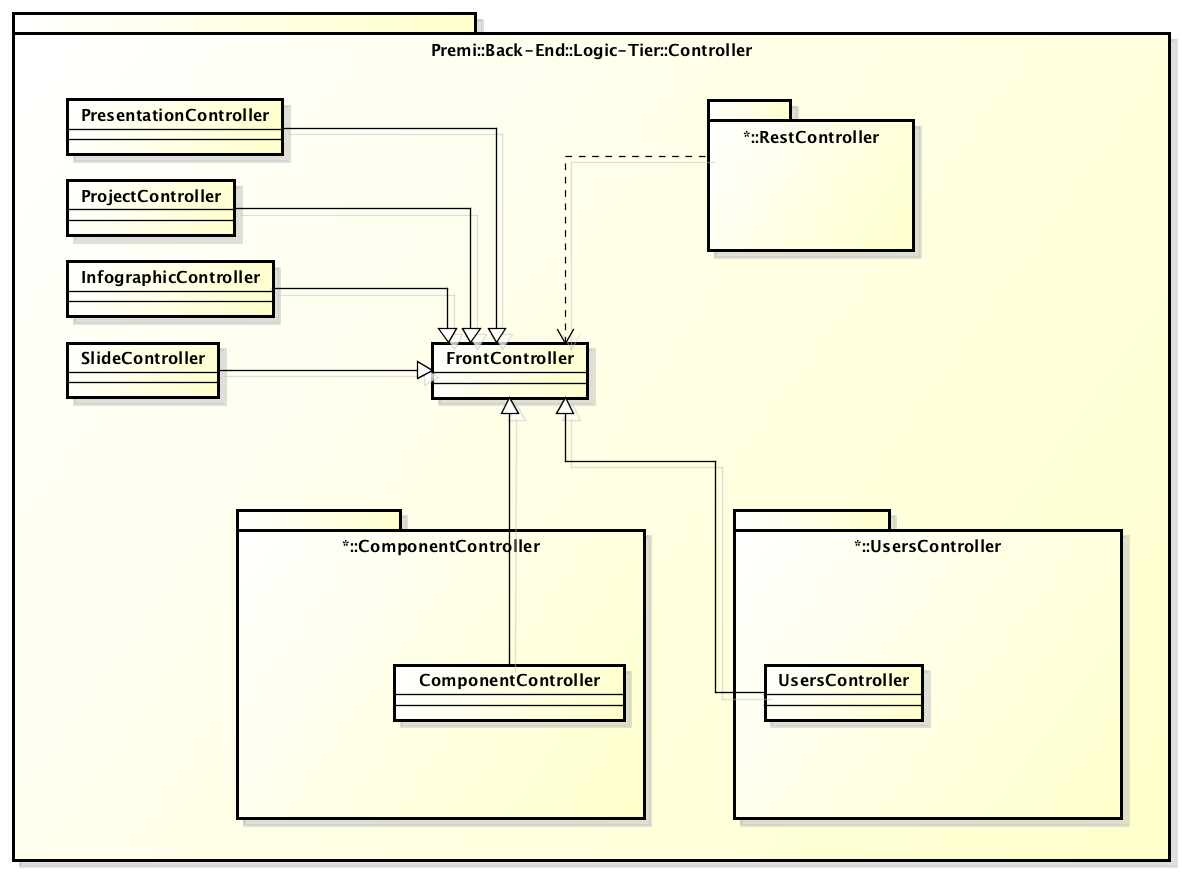
\includegraphics[width=0.9\linewidth]{img/back-end_logic-tier_controller}
		\caption[Premi::Back-End::Logic-Tier::Controller]{Premi::Back-End::Logic-Tier::Controller}
	\end{figure}
	Il package contiene le componenti che gestiscono la parte controller del lato back-end dell'applicazione. Al suo interno è presente l'interfaccia comune \textit{FrontController} dalla quale derivano tutti i controller del programma.
	Sono presenti i controller per il progetto e i suoi componenti.

	\subsubsection*{Package contenuti}
		\begin{itemize}
			\item Premi::Back-End::Logic-Tier::Controller::ComponentController:
			\begin{itemize}
				\item Descrizione: Il package contiene i controller per la gestione degli elementi di una slide.
			\end{itemize}
			
			\item Premi::Back-End::Logic-Tier::Controller::RestController:
			\begin{itemize}
				\item Descrizione: Il package contiene i controller per il REST.
			\end{itemize}
			
			\item Premi::Back-End::Logic-Tier::Controller::UsersController:
			\begin{itemize}
				\item Descrizione: Il package contiene gli elementi di controller per la gestione delle funzioni per l'utente, come login, registrazione, ricerca, ecc.
			\end{itemize}
		\end{itemize}
		
	\subsubsection*{Classi contenute}
		\begin{itemize}
			\item Premi::Back-End::Logic-Tier::Controller::FrontController:
			\begin{itemize}
				\item \textbf{Descrizione}: Classe che gestisce le operazioni e la logica applicativa degli elementi del progetto.
				\item \textbf{Relazioni con altri package}:
				\begin{itemize}
					\item Premi::Back-End::Presentation-Tier::Rest.
				\end{itemize}
			\end{itemize}
			
			\item Premi::Back-End::Logic-Tier::Controller::ProjectController:
			\begin{itemize}
				\item \textbf{Descrizione}: Classe che gestisce le operazioni e la logica riguardante la gestione e la modifica di un progetto;
				\item \textbf{Relazioni con altre classi}:
				\begin{itemize}
					\item Premi::Back-End::Logi-Tier::Controller::FrontController.
				\end{itemize}
			\end{itemize}
			
			\item Premi::Back-End::Logic-Tier::Controller::PresentationController:
			\begin{itemize}
				\item \textbf{Descrizione}: Classe che gestisce le operazioni e la logica riguardante la gestione e la modifica di una presentazione;
				\item \textbf{Relazioni con altre classi}:
				\begin{itemize}
					\item Premi::Back-End::Logi-Tier::Controller::FrontController.
				\end{itemize}
			\end{itemize}
			
			\item Premi::Back-End::Logic-Tier::Controller::InfographicController:
			\begin{itemize}
				\item \textbf{Descrizione}: Classe che gestisce le operazioni e la logica riguardante la gestione e la modifica di un'infografica;
				\item \textbf{Relazioni con altre classi}:
				\begin{itemize}
					\item Premi::Back-End::Logi-Tier::Controller::FrontController.
				\end{itemize}
			\end{itemize}
			
			\item Premi::Back-End::Logic-Tier::Controller::SlideController:
			\begin{itemize}
				\item \textbf{Descrizione}: classe che gestisce le operazioni e la logica riguardante la gestione e la modifica di una slide;
				\item \textbf{Relazioni con altre classi}:
				\begin{itemize}
					\item Premi::Back-End::Logi-Tier::Controller::FrontController.
				\end{itemize}
			\end{itemize}
		\end{itemize}
		
	
\subsection{Premi::Back-End::Logic-Tier::Controller::ComponentController}
	\subsubsection*{Informazioni sul package}
		\begin{figure}[h]
			\centering
			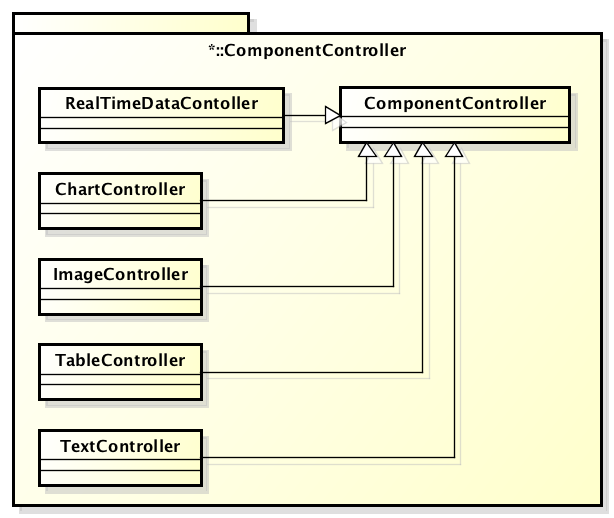
\includegraphics[width=0.9\linewidth]{img/back-end_logic-tier_controller_componentController}
			\caption[Premi::Back-End::Logic-Tier::Controller::ComponentController]{Premi::Back-End::Logic-Tier::Controller::ComponentController}
		\end{figure}
		Il package contiene le classi dei controller per la gestione degli elementi di una slide.
		
	\subsubsection*{Classi contenute}
	\begin{itemize}
		\item Premi::Back-End::Logic-Tier::Controller::ComponentController::ComponentController:
		\begin{itemize}
			\item \textbf{Descrizione}: classe che gestisce le operazioni e la logica applicativa di tutti i componenti della slide;
			\item \textbf{Relazioni con altre classi}:
			\begin{itemize}
				\item Premi::Back-End::Logic-Tier::Controller::FrontController.
			\end{itemize}
		\end{itemize}
		
		\item Premi::Back-End::Logic-Tier::Controller::ComponentController::RealTimeDataController:
		\begin{itemize}
			\item \textbf{Descrizione}: classe che gestisce le operazioni e la logica applicativa dei componenti per i dati real-time della slide;
			\item \textbf{Relazioni con altre classi}:
			\begin{itemize}
				\item Premi::Back-End::Logic-Tier::Controller::ComponentController::ComponentController.
			\end{itemize}
		\end{itemize}
		
		\item Premi::Back-End::Logic-Tier::Controller::ComponentController::ChartController:
		\begin{itemize}
			\item \textbf{Descrizione}: classe che gestisce le operazioni e la logica applicativa dei componenti per i grafici della slide;
			\item \textbf{Relazioni con altre classi}:
			\begin{itemize}
				\item Premi::Back-End::Logic-Tier::Controller::ComponentController::ComponentController.
			\end{itemize}
		\end{itemize}
		
		\item Premi::Back-End::Logic-Tier::Controller::ComponentController::ImageController:
		\begin{itemize}
			\item \textbf{Descrizione}: classe che gestisce le operazioni e la logica applicativa dei componenti per le immagini della slide;
			\item \textbf{Relazioni con altre classi}:
			\begin{itemize}
				\item Premi::Back-End::Logic-Tier::Controller::ComponentController::ComponentController.
			\end{itemize}
		\end{itemize}
		
		\item Premi::Back-End::Logic-Tier::Controller::ComponentController::TableController:
		\begin{itemize}
			\item \textbf{Descrizione}: classe che gestisce le operazioni e la logica applicativa dei componenti per le tabelle della slide;
			\item \textbf{Relazioni con altre classi}:
			\begin{itemize}
				\item Premi::Back-End::Logic-Tier::Controller::ComponentController::ComponentController.
			\end{itemize}
		\end{itemize}
		
		\item Premi::Back-End::Logic-Tier::Controller::ComponentController::TextController:
		\begin{itemize}
			\item \textbf{Descrizione}: classe che gestisce le operazioni e la logica applicativa dei componenti per le caselle di testo della slide;
			\item \textbf{Relazioni con altre classi}:
			\begin{itemize}
				\item Premi::Back-End::Logic-Tier::Controller::ComponentController::ComponentController.
			\end{itemize}
		\end{itemize}
	\end{itemize}
	
	
\subsection{Premi::Back-End::Logic-Tier::Controller::UsersController}
	\subsubsection*{Informazioni sul package}
		\begin{figure}[h]
			\centering
			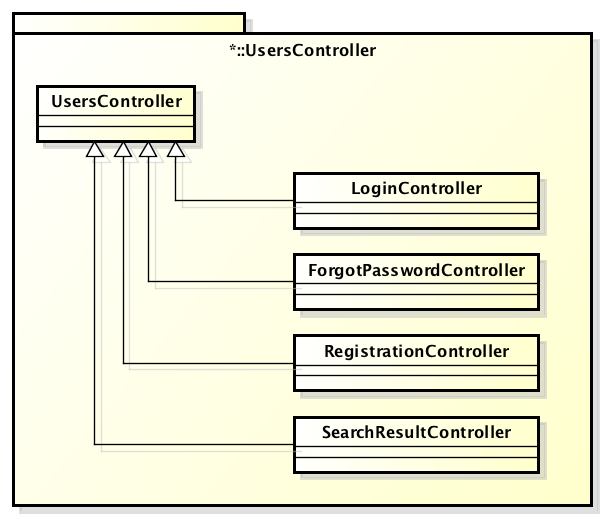
\includegraphics[width=0.9\linewidth]{img/back-end_logic-tier_controller_usersController}
			\caption[Premi::Back-End::Logic-Tier::Controller::UsersController]{Premi::Back-End::Logic-Tier::Controller::UsersController}
		\end{figure}
	Il package contiene le classi dei controller per la gestione degli utenti e le loro informazioni.
	
	\subsubsection*{Classi contenute}
		\begin{itemize}
			\item Premi::Back-End::Logic-Tier::Controller::UsersController::UsersController:
			\begin{itemize}
				\item \textbf{Descrizione}: classe che gestisce le operazioni e la logica applicativa di tutte le funzioni per la gestione di un utente e dei suoi dati;
				\item \textbf{Relazioni con altre classi}:
				\begin{itemize}
					\item Premi::Back-End::Logic-Tier::Controller::FrontController;
					\item Premi::Back-End::Logic-Tier::Model::User.
				\end{itemize}
			\end{itemize}
			
			\item Premi::Back-End::Logic-Tier::Controller::UsersController::LoginController:
			\begin{itemize}
				\item \textbf{Descrizione}: classe che gestisce le operazioni e la logica applicativa delle funzioni per il login di utente;
				\item \textbf{Relazioni con altre classi}:
				\begin{itemize}
					\item Premi::Back-End::Logic-Tier::Controller::UsersController::UsersController.
				\end{itemize}
			\end{itemize}
			
			\item Premi::Back-End::Logic-Tier::Controller::UsersController::ForgotPasswordController:
			\begin{itemize}
				\item \textbf{Descrizione}: classe che gestisce le operazioni e la logica applicativa per il recupero della password di un utente;
				\item \textbf{Relazioni con altre classi}:
				\begin{itemize}
					\item Premi::Back-End::Logic-Tier::Controller::UsersController::UsersController.
				\end{itemize}
			\end{itemize}
			
			\item Premi::Back-End::Logic-Tier::Controller::UsersController::RegistrationController:
			\begin{itemize}
				\item \textbf{Descrizione}: classe che gestisce le operazioni e la logica applicativa delle funzioni per la registrazione di un nuovo utente;
				\item \textbf{Relazioni con altre classi}:
				\begin{itemize}
					\item Premi::Back-End::Logic-Tier::Controller::UsersController::UsersController.
				\end{itemize}
			\end{itemize}
			
			\item Premi::Back-End::Logic-Tier::Controller::UsersController::SearchResultController:
			\begin{itemize}
				\item \textbf{Descrizione}: classe che gestisce le operazioni e la logica applicativa delle funzioni per la ricerca e la gestione dei risultati;
				\item \textbf{Relazioni con altre classi}:
				\begin{itemize}
					\item Premi::Back-End::Logic-Tier::Controller::UsersController::UsersController.
				\end{itemize}
			\end{itemize}
		\end{itemize}


\subsection{Premi::Back-End::Logic-Tier::Model}
	\subsubsection*{Informazioni sul package}
		\begin{figure}[h]
			\centering
			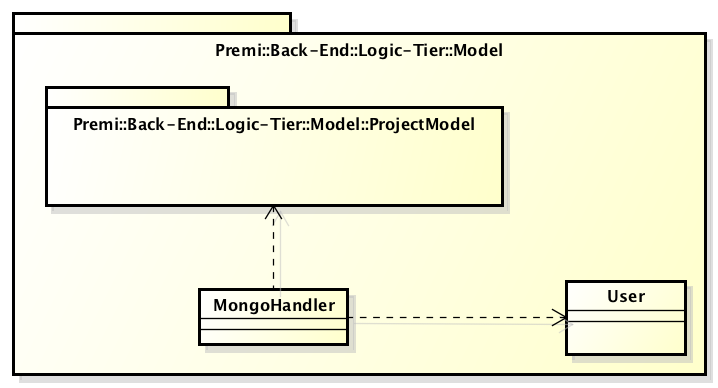
\includegraphics[width=0.9\linewidth]{img/back-end_logic-tier_model}
			\caption[Premi::Back-End::Logic-Tier::Model]{Premi::Back-End::Logic-Tier::Model}
		\end{figure}
		Il package contiene le classi che definisco il modello dell'applicazione.
	
	\subsubsection*{Package Contenuti}
		\begin{itemize}
			\item Premi::Back-End::Logic-Tier::Model::ProjectModel.
		\end{itemize}
	
	\subsubsection*{Classi contenute}
	\begin{itemize}
		\item Premi::Back-End::Logic-Tier::Model::MongoHandler:
		\begin{itemize}
			\item \textbf{Descrizione}: classe per comunicare con il livello inferiore ed interagire direttamente con la base di dati;
			\item \textbf{Relazione con altre classi}:
			\begin{itemize}
				\item Premi::Back-End::Logic-Tier::Controller::UsersController::UserController.
			\end{itemize}
		\end{itemize}
			
		\item Premi::Back-End::Logic-Tier::Model::Utente:
		\begin{itemize}
			\item \textbf{Descrizione}: classe che fornisce le operazioni per gestire un utente;
			\item \textbf{Relazione con altre classi}:
			\begin{itemize}
				\item Premi::Back-End::Data-Tier::DataTierFrontController.
			\end{itemize}
		\end{itemize}
	\end{itemize}


\subsection{Premi::Back-End::Logic-Tier::Model::ProjectModel}
	\subsubsection*{Informazioni sul package}
		\begin{figure}[h]
			\centering
			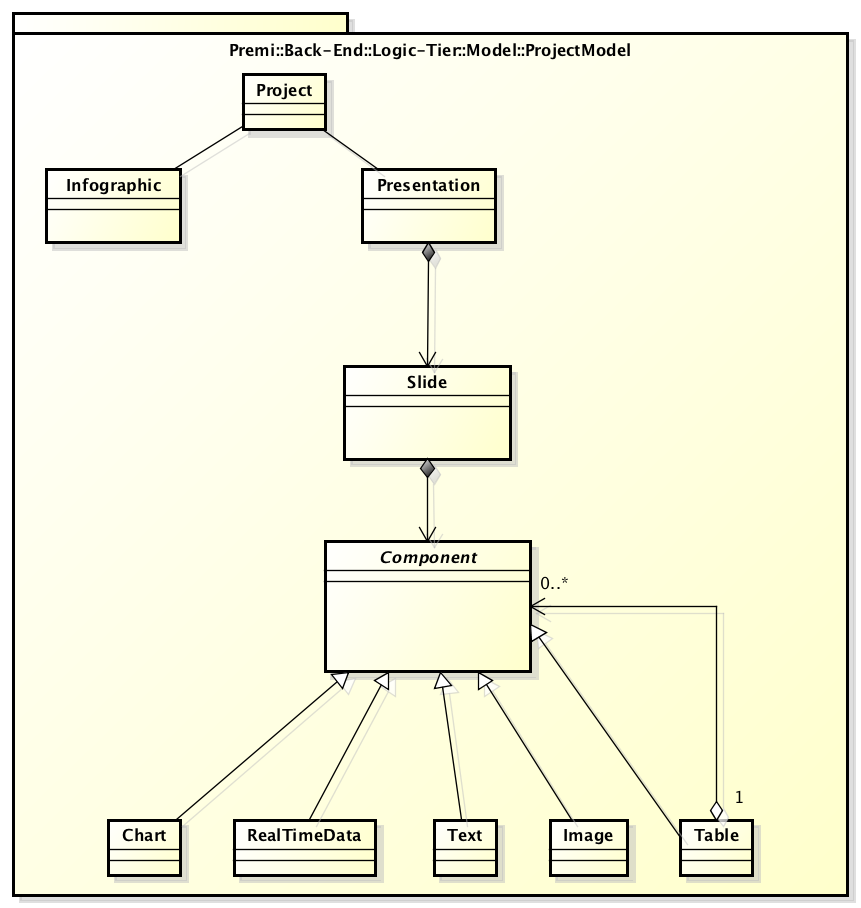
\includegraphics[width=0.9\linewidth]{img/back-end_logic-tier_model_project-model}
			\caption[Premi::Back-End::Logic-Tier::Model::ProjectModel]{Premi::Back-End::Logic-Tier::Model::ProjectModel}
		\end{figure}
		Il package contiene la struttura delle classi di tutti i componenti dell'applicazione.
	
	\subsubsection*{Classi contenute}
	\begin{itemize}
		\item Premi::Back-End::Logic-Tier::Model::ProjectModel::Project:
		\begin{itemize}
			\item \textbf{Descrizione}: classe base contenente le informazioni principali del progetto.
		\end{itemize}
			
		\item Premi::Back-End::Logic-Tier::Model::ProjectModel::Infographic:
		\begin{itemize}
			\item \textbf{Descrizione:} classe che rappresenta le infografiche associate a un progetto;
			\item \textbf{Relazione con altre classi}:
			\begin{itemize}
				\item Premi::Back-End::Logic-Tier::Model::ProjectModel::Project.
			\end{itemize}
		\end{itemize}
		
		\item Premi::Back-End::Logic-Tier::Model::ProjectModel::Presentation:
		\begin{itemize}
			\item \textbf{Descrizione:} classe che rappresenta la presentazione del progetto;
			\item \textbf{Relazione con altre classi}:
			\begin{itemize}
				\item Premi::Back-End::Logic-Tier::Model::ProjectModel::Project.
			\end{itemize}
		\end{itemize}
		
		\item Premi::Back-End::Logic-Tier::Model::ProjectModel::Slide:
		\begin{itemize}
			\item \textbf{Descrizione:} classe che rappresenta le slide che compongono una presentazione;
			\item \textbf{Relazione con altre classi}:
			\begin{itemize}
				\item Premi::Back-End::Logic-Tier::Model::ProjectModel::Project.
			\end{itemize}
		\end{itemize}
		
		\item Premi::Back-End::Logic-Tier::Model::ProjectModel::Component:
		\begin{itemize}
			\item \textbf{Descrizione:} classe base che rappresenta i componenti di cui è formata una slide;
			\item \textbf{Relazione con altre classi}:
			\begin{itemize}
				\item Premi::Back-End::Logic-Tier::Model::ProjectModel::Project.
			\end{itemize}
		\end{itemize}
		
		\item Premi::Back-End::Logic-Tier::Model::ProjectModel::Chart:
		\begin{itemize}
			\item \textbf{Descrizione:} classe che rappresenta l'elemento "grafico" che può essere inserito in una slide;
			\item \textbf{Relazione con altre classi}:
			\begin{itemize}
				\item Premi::Back-End::Logic-Tier::Model::ProjectModel::Project.
			\end{itemize}
		\end{itemize}
		
		\item Premi::Back-End::Logic-Tier::Model::ProjectModel::RealTimeData:
		\begin{itemize}
			\item \textbf{Descrizione:} classe che rappresenta l'elemento "dati real-time" che può essere inserito in una slide;
			\item \textbf{Relazione con altre classi}:
			\begin{itemize}
				\item Premi::Back-End::Logic-Tier::Model::ProjectModel::Project.
			\end{itemize}
		\end{itemize}
		
		\item Premi::Back-End::Logic-Tier::Model::ProjectModel::Text:
		\begin{itemize}
			\item \textbf{Descrizione:} classe che rappresenta l'elemento "testo" che può essere inserito in una slide;
			\item \textbf{Relazione con altre classi}:
			\begin{itemize}
				\item Premi::Back-End::Logic-Tier::Model::ProjectModel::Project.
			\end{itemize}
		\end{itemize}
		
		\item Premi::Back-End::Logic-Tier::Model::ProjectModel::Image:
		\begin{itemize}
			\item \textbf{Descrizione:} classe che rappresenta l'elemento "immagine" che può essere inserito in una slide;
			\item \textbf{Relazione con altre classi}:
			\begin{itemize}
				\item Premi::Back-End::Logic-Tier::Model::ProjectModel::Project.
			\end{itemize}
		\end{itemize}
		
		\item Premi::Back-End::Logic-Tier::Model::ProjectModel::Table:
		\begin{itemize}
			\item \textbf{Descrizione:} classe che rappresenta l'elemento "tabella" che può essere inserito in una slide;
			\item \textbf{Relazione con altre classi}:
			\begin{itemize}
				\item Premi::Back-End::Logic-Tier::Model::ProjectModel::Project.
			\end{itemize}
		\end{itemize}
	\end{itemize}


\subsection{Premi::Back-End::Data-Tier}
	\subsubsection*{Informazioni sul package}
		\begin{figure}[h]
			\centering
			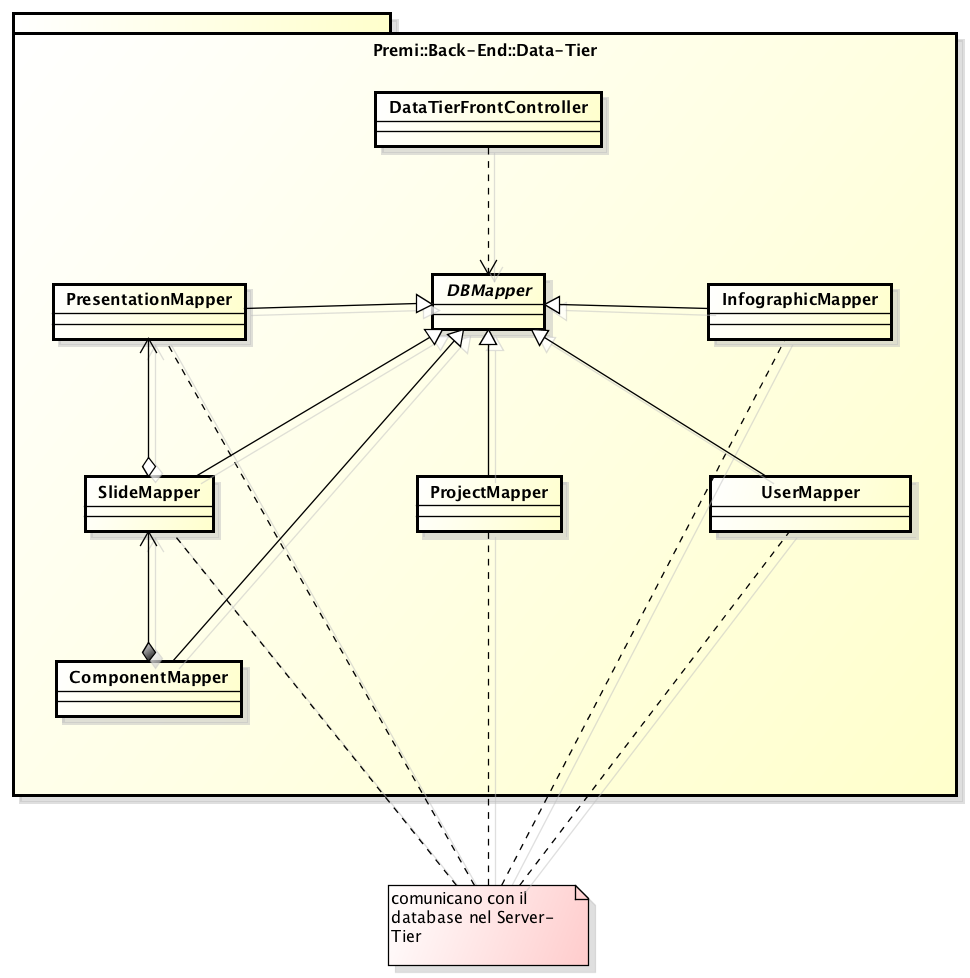
\includegraphics[width=0.9\linewidth]{img/back-end_data-tier}
			\caption[Premi::Back-End::Data-Tier]{Premi::Back-End::Data-Tier}
		\end{figure}
		Il package contiene le componenti che gestiscono l'interazione con il tier per la gestione dei dati consistenti.
		
		\subsubsection*{Classi contenute}
		\begin{itemize}
			\item Premi::Back-End::Data-Tier::DataTierFrontController:
				\begin{itemize}
					\item \textbf{Descrizione}: classe per interagire con il livello superiore e ricevere i dati dal model;
					\item \textbf{Relazione con altre classi}:
					\begin{itemize}
						\item Premi::Back-End::Logic-Tier::Model::ProjectModel::MongoHandler.
					\end{itemize}
				\end{itemize}
			
			\item Premi::Back-End::Data-Tier::DataTierFrontController:
				\begin{itemize}
					\item \textbf{Descrizione}: classe per interagire con il livello superiore e ricevere i dati dal model;
					\item \textbf{Relazione con altre classi}:
					\begin{itemize}
						\item Premi::Back-End::Logic-Tier::Model::ProjectModel::MongoHandler;
						\item Premi::Back-End::Data-Tier::DBMapper.
					\end{itemize}
				\end{itemize}
				
			\item Premi::Back-End::Data-Tier::ProjectMapper:
			\begin{itemize}
				\item \textbf{Descrizione}: classe mapper per il caricamento e il salvataggio di oggetti di tipo progetto nel database.
				\item \textbf{Relazione con altre classi}:
				\begin{itemize}
					\item Premi::Back-End::Data-Tier::DBMapper.
				\end{itemize}
			\end{itemize}
				
			\item Premi::Back-End::Data-Tier::PresentationMapper:
			\begin{itemize}
				\item \textbf{Descrizione}: classe mapper per il caricamento e il salvataggio di oggetti di tipo presentazione nel database.
				\item \textbf{Relazione con altre classi}:
				\begin{itemize}
					\item Premi::Back-End::Data-Tier::DBMapper.
				\end{itemize}
			\end{itemize}
			
			\item Premi::Back-End::Data-Tier::SlideMapper:
			\begin{itemize}
				\item \textbf{Descrizione}: classe mapper per il caricamento e il salvataggio di oggetti di tipo slide nel database.
				\item \textbf{Relazione con altre classi}:
				\begin{itemize}
					\item Premi::Back-End::Data-Tier::DBMapper.
				\end{itemize}
			\end{itemize}
			
			\item Premi::Back-End::Data-Tier::ComponentMapper:
			\begin{itemize}
				\item \textbf{Descrizione}: classe mapper per il caricamento e il salvataggio di oggetti componenti della slide nel database. Da questa classe deriveranno le altre classi specifiche per ogni componente, seguendo la struttura descritta all'interno del package *::ProjectModel;
				\item \textbf{Relazione con altre classi}:
				\begin{itemize}
					\item Premi::Back-End::Data-Tier::DBMapper.
				\end{itemize}
			\end{itemize}
			
			\item Premi::Back-End::Data-Tier::InfographicMapper:
			\begin{itemize}
				\item \textbf{Descrizione}: classe mapper per il caricamento e il salvataggio di oggetti di tipo infografica nel database.
				\item \textbf{Relazione con altre classi}:
				\begin{itemize}
					\item Premi::Back-End::Data-Tier::DBMapper.
				\end{itemize}
			\end{itemize}
			
			\item Premi::Back-End::Data-Tier::UserMapper:
			\begin{itemize}
				\item \textbf{Descrizione}: classe mapper per il caricamento e il salvataggio di oggetti di tipo utente nel database.
				\item \textbf{Relazione con altre classi}:
				\begin{itemize}
					\item Premi::Back-End::Data-Tier::DBMapper.
				\end{itemize}
			\end{itemize}
		\end{itemize}
		

\subsection{Scenari}
\subsubsection{Gestione richiesta di registrazione}
Il seguente diagramma rappresenta lo scenario con il quale viene gestita una richiesta di registrazione. La richiesta viene gestita da \textit{RegistrationController} che controlla il corretto inserimento dei dati e invia il responso a \textit{UsersController}, il quale può agire in due modi diversi: se la richiesta é stata fatta correttamente allora invia un CreateUser() a Utenti per creare il nuovo utente, avvisa \textit{RegistrationController} che la registrazione é avvenuta tramite RegistrationDone() e viene emanato un segnale di Redirect(); se la richiesta ha prodotto degli errori viene inviato un RegistrationError() a \textit{RegistrationController} che comunica l'errore per mezzo di un ErrorMessage().
\begin{figure}[H]
	\centering
	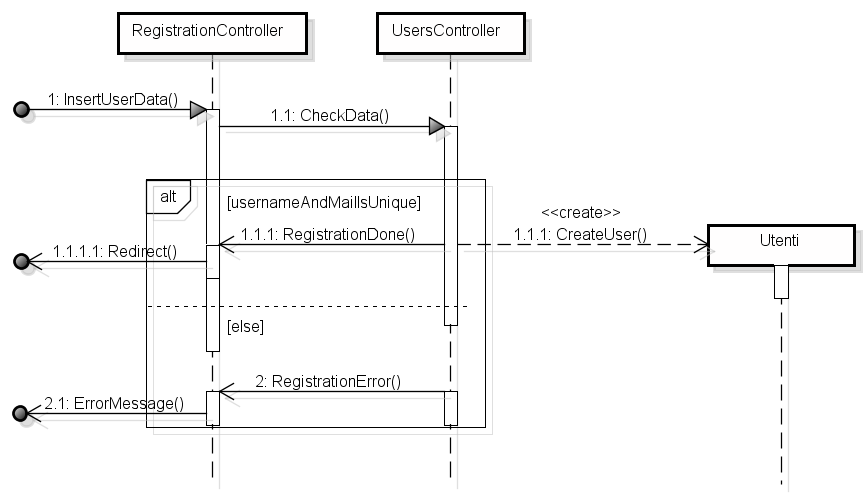
\includegraphics[scale=0.5]{img/register.png}
	\caption{Diagrammi di sequenza - Richiesta di registrazione}
\end{figure}

\subsubsection{Gestione richiesta di autenticazione}
Il seguente diagramma rappresenta lo scenario con il quale viene gestita una richiesta di autenticazione. La richiesta viene presa in carico da \textit{LoginController} che verifica i dati e invia un CheckData() a \textit{UsersController}, da qui viene inviato un SearchForUser() a \textit{Utenti} per trovare una corrispondenza. Se le credenziali sono corrette \textit{Utenti} lo segnala a \textit{UsersController} tramite CorrectCredentials() e alla fine viene emesso un segnale di Redirect(); se le credenziali non sono corrette viene segnalato l'errore con un IncorrectCredentials() e in uscita arriva un ErrorMessage().\\
Da qui è possibile che arrivi una richiesta di recupero password. Essa é gestita da \textit{LoginController} che invia un CredentialsRecoveryRequest() a \textit{ForgotPasswordController}, poi \textit{UsersController} verifica i dati ricevuti e ricerca l'utente con un SearchForUser() verso \textit{Utenti}. Se i dati per il recupero password sono corretti \textit{UsersController} invia un CredentialsSendToMail() a \textit{ForgotPasswordController}, altrimenti viene inviato un CredentialsError(). Alla fine inviato un segnale in uscita RecoveryMessage() o ErrorMessage() da \textit{LoginController} rispettivamente se il recupero credenziali ha avuto buon esito o se é fallito.

\begin{figure}[H]
	\centering
	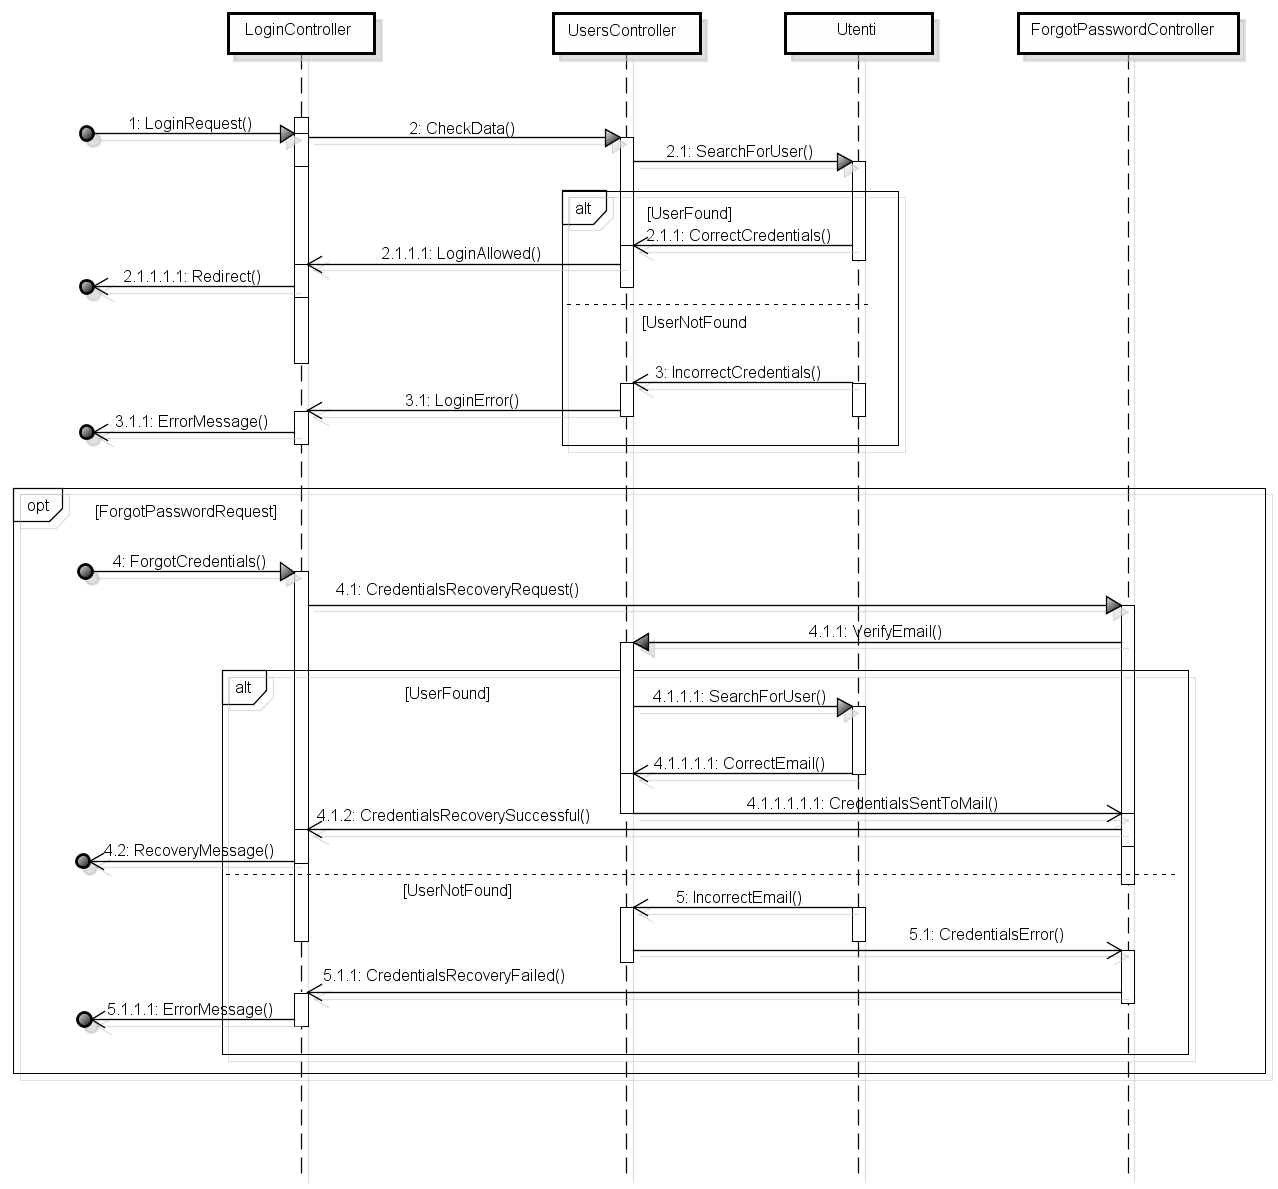
\includegraphics[scale=0.5]{img/login.png}
	\caption{Diagrammi di sequenza - Richiesta di autenticazione}
\end{figure}

\subsubsection{Gestione richiesta di ricerca di un progetto}
Il diagramma seguente rappresenta lo scenario con il quale viene gestita una richiesta di ricerca di un progetto. \textit{SearchResultController} interpreta la richiesta e definisce se sia una ricerca tramite nome utente o tramite nome del progetto. Nel primo caso viene inviato un CheckData() a \textit{UsersController} che verifica la richiesta e invia un SendResults() a \textit{SearchResultsController} che emette un DataResults(). Nel secondo caso il CheckData() viene inviato a \textit{ProjectController} che risponde con un SendResults() a \textit{SearchResultsController} che invia un DataResults().
\newpage
\begin{figure}[H]
	\centering
	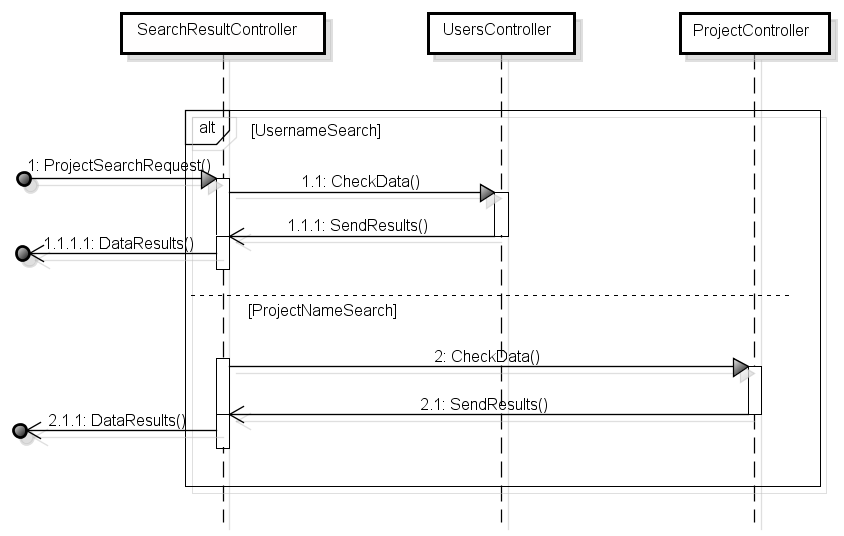
\includegraphics[scale=0.5]{img/search.png}
	\caption{Diagrammi di sequenza - Richiesta di ricerca di un progetto}
\end{figure}

\subsubsection{Gestione richiesta di visualizzazione di una presentazione}
Il diagramma seguente rappresenta lo scenario con il quale viene gestita una richiesta di visualizzazione di una presentazione. La richiesta é gestita da \textit{PresentationController} che invia un FindPresentation() a \textit{Presentation} che recupera la prima slide tramite un RetrieveFirstSlide() verso \textit{Slide}, il quale ritorna un FirstSlideFound(). Infine \textit{Presentation} segnala a \textit{PresentationController} che la visualizzazione é pronta, viene inviato un ViewingReady() a \textit{PresentationController} che ritorna un ViewingStartData().

\begin{figure}[H]
	\centering
	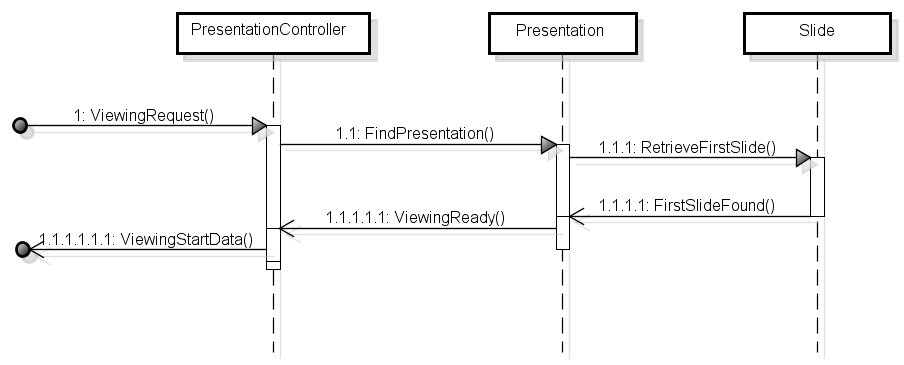
\includegraphics[scale=0.5]{img/view.png}
	\caption{Diagrammi di sequenza - Richiesta di visualizzazione di una presentazione}
\end{figure} 


\subsubsection{Gestione richiesta di creazione di un progetto}
Il seguente diagramma rappresenta lo scenario con il quale viene gestita una richiesta di creazione di un progetto. La richiesta viene gestita da \textit{ProjectController} il quale crea, tramite CreateProject(), un nuovo progetto in \textit{Project} e invia un ProjectCreatedData() di ritorno.

\begin{figure}[H]
	\centering
	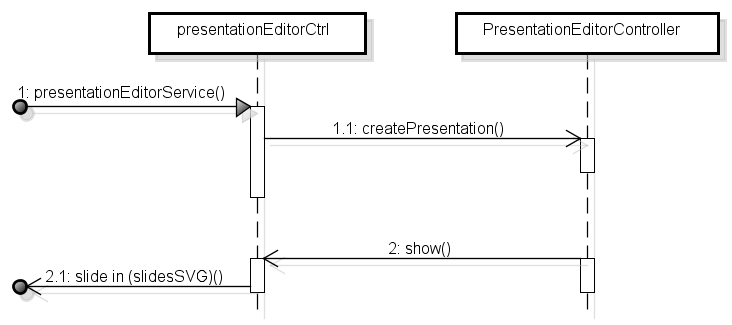
\includegraphics[scale=0.5]{img/create.png}
	\caption{Diagrammi di sequenza - Richiesta di creazione di un progetto}
\end{figure}

\subsubsection{Gestione richiesta di apertura di un progetto}
Il seguente diagramma rappresenta lo scenario con il quale viene gestita una richiesta di apertura di un progetto. La richiesta viene gestita da \textit{ProjectController} che invia un SearchForProject() a \textit{Project} per cercare il progetto richiesto. Se l'utente non interrompe l'apertura, da \textit{Project} viene inviato un ProjectFound() a \textit{ProjectController} che ritorna un OpeningProjectData(), altrimenti \textit{Project} invia un OpeningCancelled() e successivamente viene ritornato un UserInterruptMessage() da \textit{ProjectController}.

\begin{figure}[H]
	\centering
	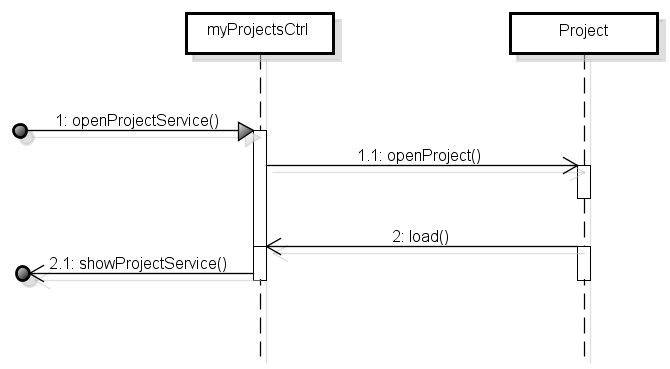
\includegraphics[scale=0.5]{img/open.png}
	\caption{Diagrammi di sequenza - Richiesta di apertura di un progetto}
\end{figure}

\newpage

\subsubsection{Gestione richiesta di modifica di un progetto}
Si é deciso di suddividere in sotto-diagrammi il diagramma riguardante la richiesta di modifica, al fine di rendere meno complicata e di più facile comprensione il diagramma stesso. A causa di questa suddivisione i diagrammi saranno tra loro molto simili, la gestione delle richieste infatti é la stessa, cambiano i componenti e il nome di alcuni segnali. Si utilizzerà la dicitura \{element\} per indicare uno degli elementi modificabili di una slide (chart, table, image, text, o real time) nella seguente spiegazione. 
\\Lo scenario generale con il quale vengono gestite le richieste é il seguente:
\begin{itemize}
	\item[]la richiesta di modifica viene gestita da \textit{\{element\}Controller} che la interpreta e invia un InterpretRequest() a \textit{ComponentController}. Nel caso riguardi la creazione di un nuovo \{element\}, \textit{ComponentController} invia un Insert\{element\}() o un Create\{element\}() a \textit{\{element\}} che crea l'elemento richiesto. Viene poi inviato un CreationDone() da \textit{ComponentController} a \textit{\{element\}Controller} che ritorna un ElDataSend().\\
	Se invece la richiesta é una richiesta di modifica \textit{ComponentController} invia un Modify\{element\} a \textit{\{element\}} che può accettare le modifiche con un \{element\}Updated() o rifiutarle con \{element\}Error(). Se vengono accettate \textit{ComponentController} invia un ModifyDone() a \textit{\{element\}Controller} che ritorna un ElDataSend(), altrimenti invia un ModifyError() e viene ritornato un MessageError().
\end{itemize}
I diagrammi verranno elencati ora uno dopo l'altro.
\newpage

\begin{figure}[H]
	\centering
	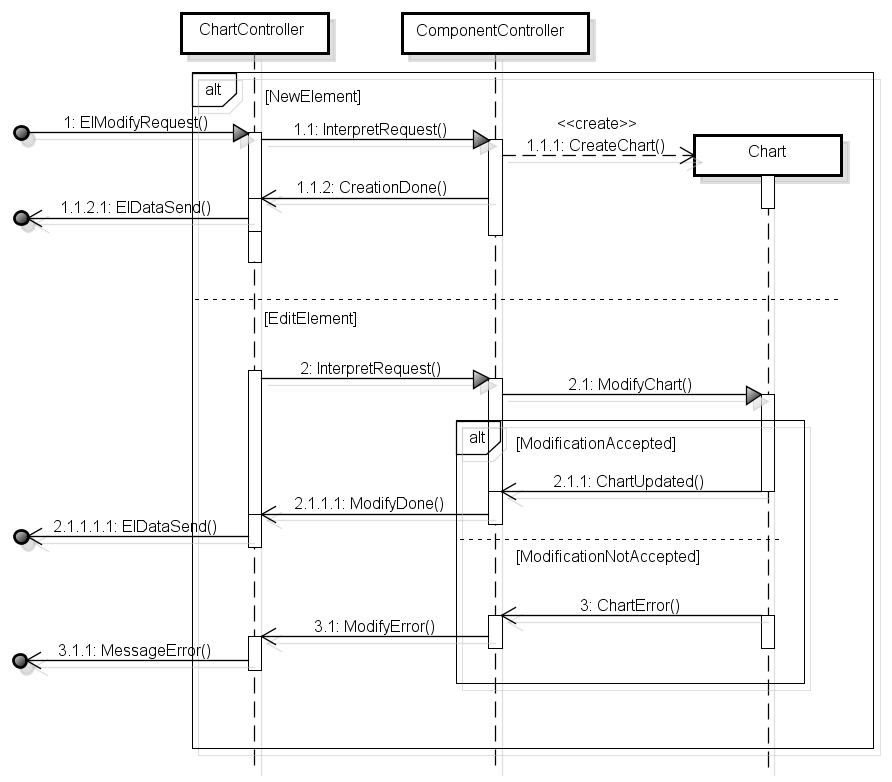
\includegraphics[scale=0.5]{img/chart.png}
	\caption{Diagrammi di sequenza - Richiesta di modifica di un progetto: grafici}
\end{figure}

\begin{figure}[H]
	\centering
	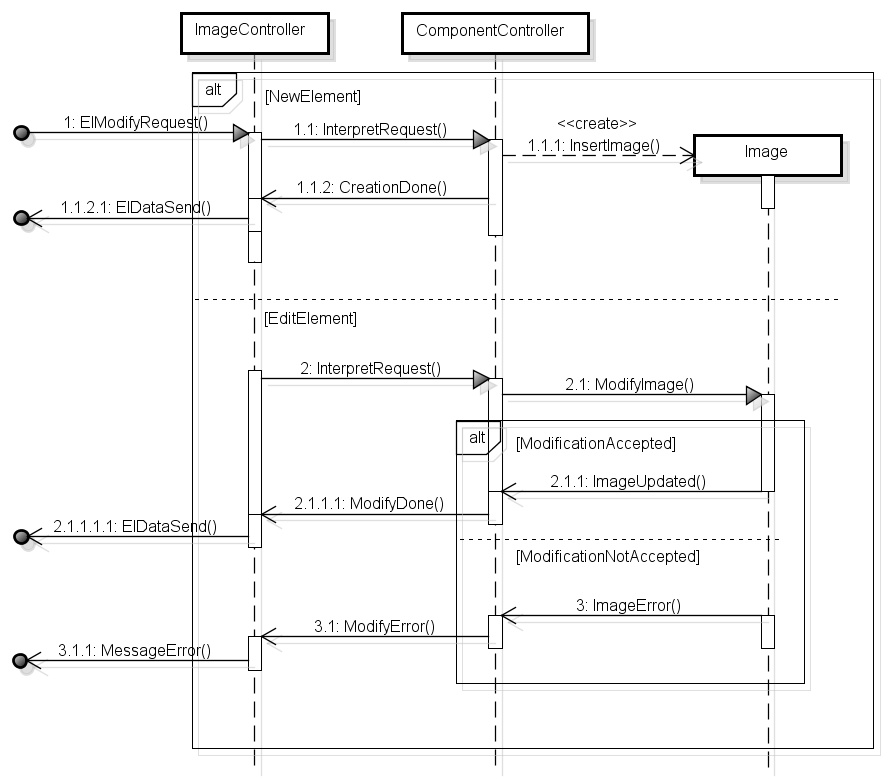
\includegraphics[scale=0.5]{img/image.png}
	\caption{Diagrammi di sequenza - Richiesta di modifica di un progetto: immagini}
\end{figure}

\begin{figure}[H]
	\centering
	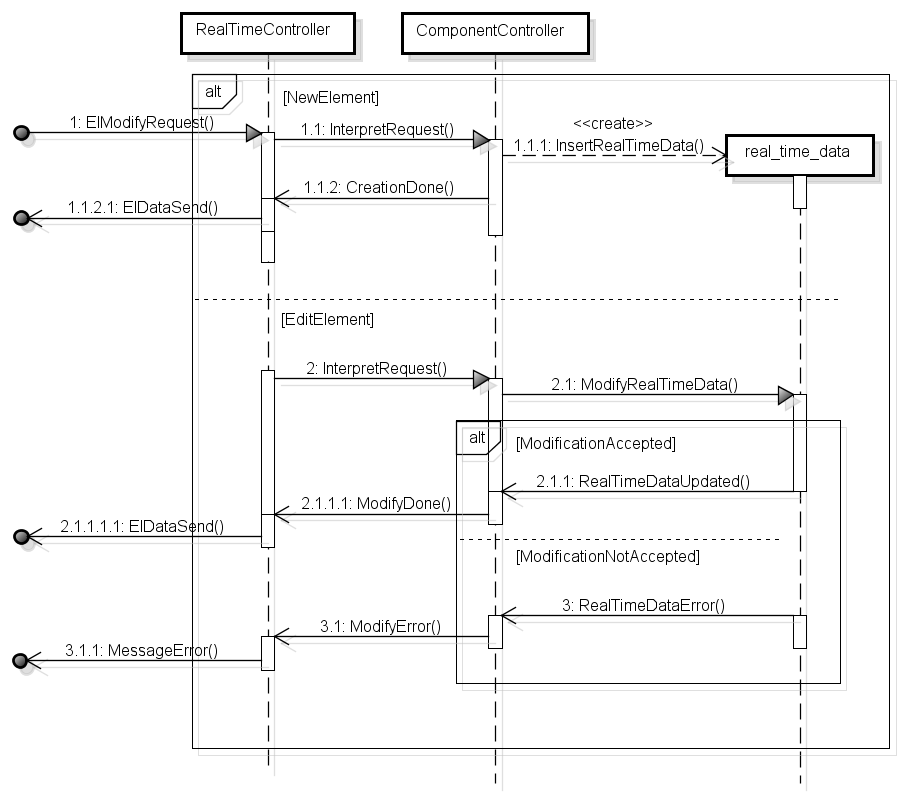
\includegraphics[scale=0.5]{img/real_time.png}
	\caption{Diagrammi di sequenza - Richiesta di modifica di un progetto: dati Real Time}
\end{figure}

\begin{figure}[H]
	\centering
	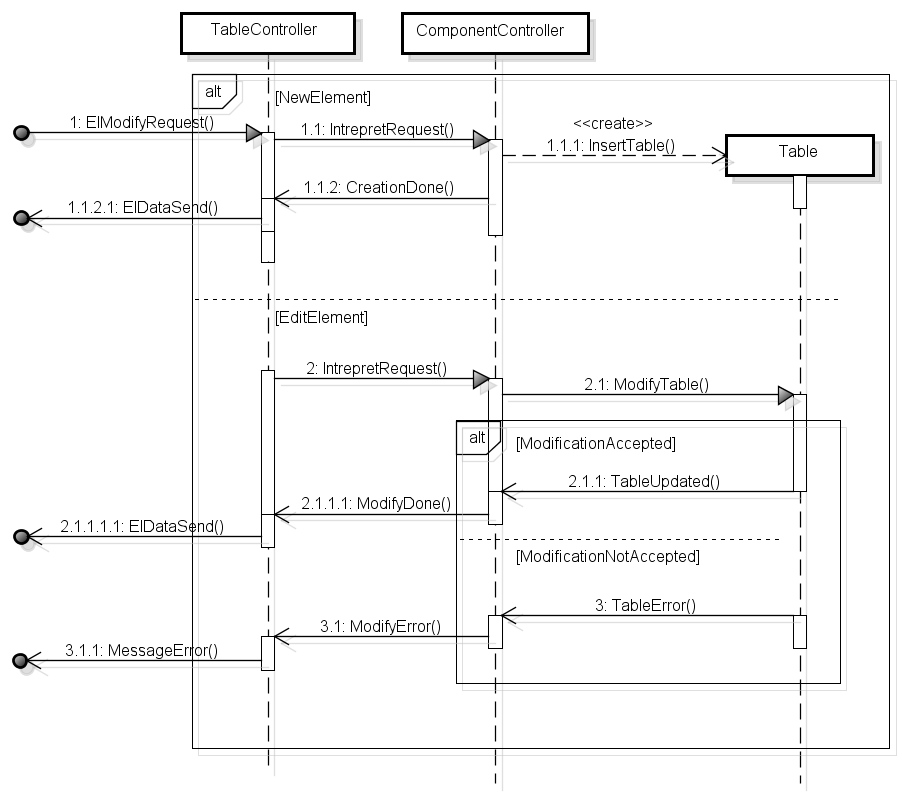
\includegraphics[scale=0.5]{img/table.png}
	\caption{Diagrammi di sequenza - Richiesta di modifica di un progetto: tabelle}
\end{figure}

\begin{figure}[H]
	\centering
	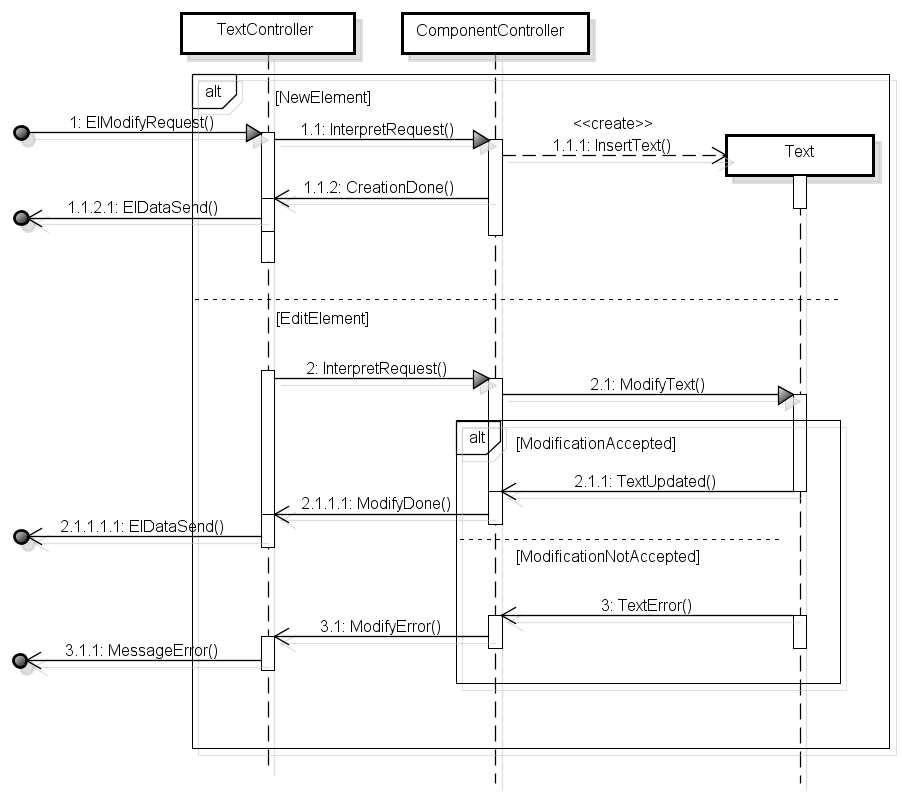
\includegraphics[scale=0.5]{img/text.png}
	\caption{Diagrammi di sequenza - Richiesta di modifica di un progetto: testi}
\end{figure}

\subsubsection{Gestione richiesta salvataggio di un progetto}
Il seguente diagramma rappresenta lo scenario con il quale viene gestita una richiesta di salvataggio di un progetto. La richiesta viene gestita da \textit{ProjectController} che invia un SavingProject() a \textit{Project}. Nel caso l'utente confermi il salvataggio viene inviato un ProjectSaved() a \textit{ProjectController} a sua volta invia un SavingData(); se l'utente interrompe il salvataggio \textit{Project} invia un SavingCancelled() a \textit{ProjectController} che ritorna un UserInterruptMessage().

\begin{figure}[H]
	\centering
	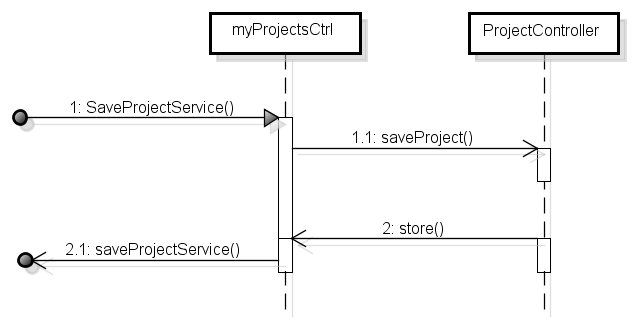
\includegraphics[scale=0.5]{img/save.png}
	\caption{Diagrammi di sequenza - Richiesta di salvataggio di un progetto}
\end{figure}
\newpage